\chapter{Conclusions and Future Work} \label{chap:conclusions}

This planning report had two distinct objectives. The first one is the search of related works in order to see what is already developed to the problem context of this dissertation. The second objective is the initial planning of the dissertation work, as well as the approach and methodology chosen to tackle the problem in hands. From the all work made so far, it is possible to make some conclusions.

This dissertation proposes to tackle the problem of extraction of aspect-based sentiment from the citizens opinions about the services of a city, in social media streams, through a framework that may be capable of processing the messages and build some appealing visual indicators.

Hence, the problem was decomposed in some sub-problems. The literature review served to find interesting solutions for each sub-problem. There, a great diversity of approaches was found, not only about sentiment analysis that is the most important task in this dissertation but also for another problems like the content filtering and disambiguation.

The proposed framework can be seen as a potential tool to the users of the city's services and for the responsible entities, allowing that only good decisions are made to improve the quality of the cities and, in this particular case, the urban transportation systems. 

To summarize the conclusions of all the work made so far, a SWOT analysis was conceived and the points that composed it are present below.

\begin{enumerate}
   \item \textbf{Strengths}
   \begin{itemize}
     \item Added value proposal by combining multiple State-of-the-Art approaches to tackle chained sub-tasks;
     \item Well defined sub-tasks/modules will make it easier to track errors.
   \end{itemize}
   \item \textbf{Weaknesses}
   \begin{itemize}
     \item It might be difficult to collect enough relevant data for specific scenarios (e.g. the quality of the urban transportation in Porto);
     \item Twitter data might not be so reliable if there are few relevant messages.
   \end{itemize}
   \textbf{Opportunities}
   \begin{itemize}
     \item New scenario application for aspect-based sentiment analysis: transportation systems and Smart Cities;
     \item Extending State-of-the-Art approaches in each sub-task/module if the target scenario presents specific constraints.
   \end{itemize}
   \textbf{Threats}
   \begin{itemize}
     \item Absence of ground-truths for the target scenarios may lead to underperformed modules;
     \item Limited time for implementation is a risk of some unforeseen difficulties arise.
   \end{itemize}
\end{enumerate}

\section{Expected Contributions}

The work to be developed in this dissertation should present contributions both at the technological and scientific level. Some of the most important contributions are listed below:

\begin{itemize}
\item A brief review of related literature to help contextualize readers in the subject of information extraction, in particular the sentiment analysis, from social media streams and how difficult is this task;
\item Development of a tool that could bring a potential value to the cities in order to improve the quality of its services;
\item The studies of use cases about Smart Cities and Transportation Systems using aspect-based sentiment analysis may be considered something innovative since there are very few works related with both scenarios.
\end{itemize}

\section{Task Planning and Scheduling}
The tasks to be undertaken are mostly based in the modules described in Section \ref{sec:architecture} for the proposed framework architecture.
The first task is to choose what are the specific scenarios that will serve to test the developed framework. A priori, two different scenarios will be enough to prove the good functionality and usability of the tool. Hence, the crawler module will be used to collect social media streams from the middle of February until, approximately, the ending of May. Meanwhile, the setup of the framework environment needs to be done. After this first step, the development of the modules will occur. The first module to tackle is the aspect-based sentiment analysis and the sub-module of preprocessing. With the estimation of a possible margin of error, these tasks are ready to employment in the begin or middle of April. The target filtering module will be developed, if everything is going as planned, between the beginning/middle of April until the middle of May. The remaining month of May will serve to work on the aggregation module and the analytics UI. The month of June will be to test the final framework into the collected dataset about the two different scenarios. In order to evaluate the usability of the framework, it's planned the existence of a bunch of interviews to see if it's really possible that users of this tool are capable of immediately identify some conclusion from the analysis presented. This evaluation step will occur in the first two weeks of June, being the remaining two to the final dissertation report write up.

In the Figure \ref{fig:workplan} it's possible to visualize a Gantt chart scheduling according the mentioned tasks and the ideal scenario in case there are no delays.

\begin{figure}
  \centering
    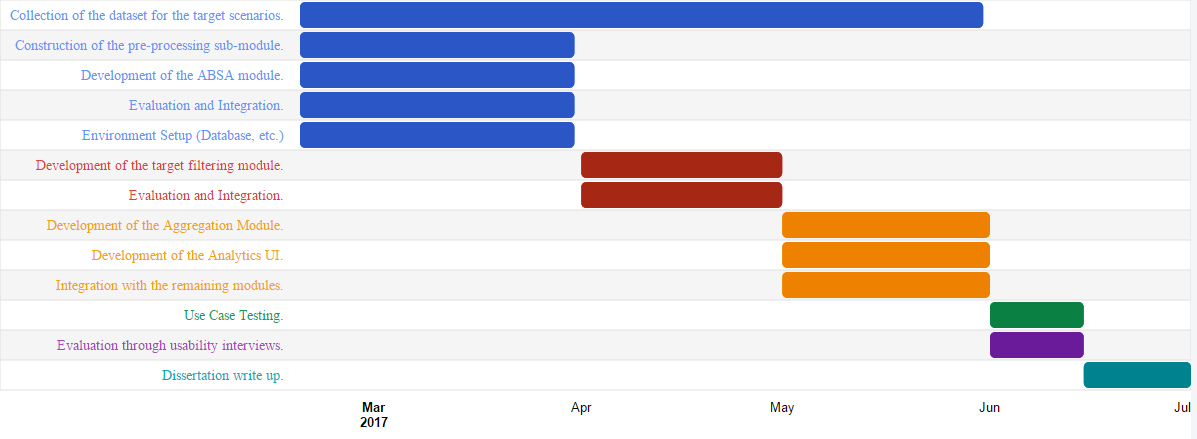
\includegraphics[width=1.1\textwidth]{workplan}
    \caption{Dissertation working plan.}
    \label{fig:workplan}
\end{figure}

\vspace*{12mm} 
